\chapter{Implementation}
%\lstinputlisting[caption=Hello World]{project/code/helloworld.py}
\textbf{Activity:}\\
\hspace*{0.82cm}An activity is a single, focused thing that the user can do. Almost all activities interact with the user, so the Activity 
class takes care of creating a window for you in which you can place your UI with \texttt{setContentView(View)}. While activities are often 
presented to the user as full-screen windows, they can also be used in other ways: as floating windows (via a theme with \texttt{windowIsFloating} 
set) or embedded inside of another activity (using \texttt{ActivityGroup}). There are two methods almost all subclasses of Activity will implement:
\begin{itemize}
 \item \textbf{onCreate(Bundle)} is where you initialize your activity. Most importantly, here you will usually call \texttt{setContentView(int)} 
with a layout resource defining your UI, and using \texttt{findViewById(int)} to retrieve the widgets in that UI that you need to interact with 
programmatically.
\item \textbf{onPause()} is where you deal with the user leaving your activity. Most importantly, any changes made by the user should at this 
point be committed (usually to the \texttt{ContentProvider} holding the data).
\end{itemize}
To be of use with \texttt{Context.startActivity()}, all activity classes must have a corresponding \texttt{<activity>} declaration in their 
package's \texttt{AndroidManifest.xml}.\\[0.5cm]

\begin{lstlisting}
  public class Activity extends ApplicationContext {
     protected void onCreate(Bundle savedInstanceState);
     protected void onStart();    
     protected void onRestart();
     protected void onResume();
     protected void onPause();
     protected void onStop();
     protected void onDestroy();
 }
\end{lstlisting}
\newpage
%\vspace*{1cm}
\begin{figure}[H]
  \centering
    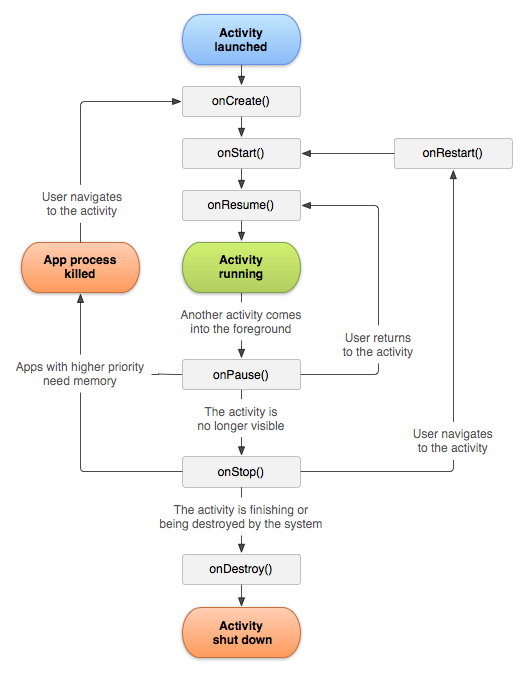
\includegraphics[scale=0.6]{project/images/activity-lifecycle}
  \caption{\textbf{Important State Paths of an Activity}}
\end{figure}
%\newpage
\textbf{Bluetooth Adapter}\\
\hspace*{0.82cm}The \texttt{BluetoothAdapter} lets you perform fundamental Bluetooth tasks, such as initiate device discovery, query a 
list of bonded (paired) devices, instantiate a \texttt{BluetoothDevice} using a known MAC address.\\[0.5cm]
\hspace*{0.82cm}Create a \texttt{BluetoothServerSocket} to listen for connection requests from other devices. 
%\\[0.5cm]
%\hspace*{0.82cm}
To get a \texttt{BluetoothAdapter} representing the local Bluetooth adapter, call the static \texttt{getDefaultAdapter()} method. 
Fundamentally, this is your starting point for all Bluetooth actions. Once you have the local adapter, you can get a set of 
\texttt{BluetoothDevice} objects representing all paired devices with \texttt{getBondedDevices()}; start device discovery with 
\texttt{startDiscovery()}.\\[0.5cm]
\hspace*{0.82cm}Create a \texttt{BluetoothServerSocket} to listen for incoming connection requests with 
\texttt{listenUsingRfcommWithServiceRecord(String, UUID)}.
\newpage
\textbf{Bluetooth Server Socket}\\
\hspace*{0.82cm}The interface for Bluetooth Sockets is similar to that of TCP sockets: \texttt{Socket} and \texttt{ServerSocket}. On the 
server side, use a \texttt{BluetoothServerSocket} to create a listening server socket. When a connection is accepted by the 
\texttt{BluetoothServerSocket}, it will return a new \texttt{BluetoothSocket} to manage the connection. On the client side, use a single 
\texttt{BluetoothSocket} to both initiate an outgoing connection and to manage the connection.\\[0.5cm]
\hspace*{0.82cm}The most common type of Bluetooth socket is RFCOMM, which is the type supported by the Android APIs. RFCOMM is a 
connection-oriented, streaming transport over Bluetooth. It is also known as the Serial Port Profile (SPP).\\[0.5cm]
\hspace*{0.82cm}To create a listening \texttt{BluetoothServerSocket} that's ready for incoming connections,  use 
\texttt{BluetoothAdapter.listenUsingRfcommWithServiceRecord()}.\\Then call \texttt{accept()} to listen for incoming connection requests. 
This call will block until a connection is established, at which point, it will return a \texttt{BluetoothSocket} to manage the connection. 
Once the \texttt{BluetoothSocket} is acquired, it's a good idea to call \texttt{close()} on the \texttt{BluetoothServerSocket} when it's no 
longer needed for accepting connections. Closing the \texttt{BluetoothServerSocket} will not close the returned \texttt{BluetoothSocket}.\\[0.5cm]
\hspace*{0.82cm}\texttt{BluetoothServerSocket} is thread safe. In particular, \texttt{close()} will always immediately abort ongoing 
operations and close the server socket.\\[1cm]
\textbf{Bluetooth Socket}\\
\hspace*{0.82cm}The interface for Bluetooth Sockets is similar to that of TCP sockets: \texttt{Socket} and \texttt{ServerSocket}. On the 
server side, use a \texttt{BluetoothServerSocket} to create a listening server socket. When a connection is accepted by the 
\texttt{BluetoothServerSocket}, it will return a new \texttt{BluetoothSocket} to manage the connection. On the client side, use a single 
\texttt{BluetoothSocket} to both initiate an outgoing connection and to manage the connection.\\[0.5cm]
\hspace*{0.82cm}The most common type of Bluetooth socket is RFCOMM, which is the type supported by the Android APIs. RFCOMM is a 
connection-oriented, streaming transport over Bluetooth. It is also known as the Serial Port Profile (SPP).\\[0.5cm]
\hspace*{0.82cm}To create a \texttt{BluetoothSocket} for connecting to a known device, use\\
\texttt{BluetoothDevice.createRfcommSocketToServiceRecord()}. Then call \texttt{connect()} to attempt a connection to the remote device. 
This call will block until a connection is established or the connection fails.\\[0.5cm]
\hspace*{0.82cm}Once the socket is connected, whether initiated as a client or accepted as a server, open the IO streams by calling 
\texttt{getInputStream()} and \texttt{getOutputStream()} in order to retrieve \texttt{InputStream} and \texttt{OutputStream} objects, 
respectively, which are automatically connected to the socket.\\[0.5cm]
\hspace*{0.82cm}\texttt{BluetoothSocket} is thread safe. In particular, \texttt{close()} will always immediately abort ongoing operations 
and close the socket.\\[1cm]
\textbf{Contacts Contract}\\
\hspace*{0.82cm}ContactsContract defines an extensible database of contact-related information. Contact information is stored in a 
three-tier data model:
\begin{itemize}
 \item A row in the \texttt{ContactsContract.Data} table can store any kind of personal data, such as a phone number or email addresses. 
The set of data kinds that can be stored in this table is open-ended. There is a predefined set of common kinds, but any application 
can add its own data kinds.
 \item A row in the \texttt{ContactsContract.RawContacts} table represents a set of data describing a person and associated with a 
single account (for example, one of the user's Gmail accounts).
 \item A row in the \texttt{ContactsContract.Contacts} table represents an aggregate of one or more RawContacts presumably describing 
the same person. When data in or associated with the RawContacts table is changed, the affected aggregate contacts are updated as necessary. 
\end{itemize}
\vspace{1cm}
\textbf{Content Provider}\\
\hspace*{0.82cm}Content providers are one of the primary building blocks of Android applications, providing content to applications. 
They encapsulate data and provide it to applications through the single \texttt{ContentResolver} interface. A content provider is only 
required if you need to share data between multiple applications. For example, the contacts data is used by multiple applications and 
must be stored in a content provider. If you don't need to share data amongst multiple applications you can use a database directly via 
\texttt{SQLiteDatabase}.\\[0.5cm]
\hspace*{0.82cm}When a request is made via a \texttt{ContentResolver} the system inspects the authority of the given URI and passes the 
request to the content provider registered with the authority. The content provider can interpret the rest of the URI however it wants. 
The \texttt{UriMatcher} class is helpful for parsing URIs.\\[0.5cm]
The primary methods that need to be implemented are:
\begin{itemize}
 \item \texttt{onCreate()} which is called to initialize the provider
 \item \texttt{query(Uri, String[], String, String[], String)} which returns data to the caller
 \item \texttt{insert(Uri, ContentValues)} which inserts new data into the content provider
 \item \texttt{update(Uri, ContentValues, String, String[])} which updates existing data in the content provider
 \item \texttt{delete(Uri, String, String[])} which deletes data from the content provider
 \item \texttt{getType(Uri)} which returns the MIME type of data in the content provider
\end{itemize}
\hspace*{0.82cm}Requests to \texttt{ContentResolver} are automatically forwarded to the appropriate \texttt{ContentProvider} instance, 
so subclasses don't have to worry about the details of cross-process calls.\\[1cm]
\textbf{Telephony Manager}\\
\hspace*{0.82cm}Provides access to information about the telephony services on the device. Applications can use the methods in this class to 
determine telephony services and states, as well as to access some types of subscriber information. Applications can also register a listener 
to receive notification of telephony state changes.\\[0.5cm]
\hspace*{0.82cm}You do not instantiate this class directly; instead, you retrieve a reference to an instance through 
\texttt{Context.getSystemService(Context.TELEPHONY\_SERVICE)}.\\[0.5cm]
\hspace*{0.82cm}Note that access to some telephony information is permission-protected. Your application cannot access the protected 
information unless it has the appropriate permissions declared in its manifest file. Where permissions apply, they are noted in the 
the methods through which you access the protected information.